\documentclass[11pt]{article}

\usepackage{graphicx}
\usepackage{url}
\usepackage{amsmath}

\title{VisibleSim Manual}
\author{Julien Bourgeois, Benoît Piranda, Thadeu Knychala Tucci, André Naz}

\begin{document}

\maketitle

\newpage
\tableofcontents
\newpage

\section{Introduction}

VisibleSim is a general discrete event simulator (DES) for modular robot systems.

\section{Installation}

\section{User applications in VisibleSim}

\subsection{Examples of applications}

\subsection{Implementing a new application}

\subsection{Running an application}
\subsubsection{C++ application}
\subsubsection{Meld application}
\subsubsection{Command line arguments}

\section{Embedded debugger}

\section{Local clock Simulation}

VisibleSim supports local clock simulation. We present here the programming API and the clock model. The model

\subsection{Programming API}

\subsection{Clock model}

We used hardware Blinky Blocks to compute realistic clock models. Blinky Blocks are eqquiped with a micro-controller ATxmega256A3 that holds a 16-bit Real Time Xounter (RTC). The RTC can be plugged to different oscillators. We choose to study clock behaviour using the most precise internal oscillator available: a 32.768 kHz calibrated RC oscillator with a precision of 1\% and a resolution of 1 ms.

RC oscillator are known to drift apart linearly.
Voltage 

The set of blocks were powered with 5V and 0.36A. 

\subsubsection{Systematic model for clocks}

\cite{allan1987time} proposes a general model for oscillators:
\begin{equation}
x(t) = x_0 + y_0t + \frac{1}{2}Dt^2 + \epsilon(t)
\end{equation}
where $t$ is the simulation time (real-time), $x(t)$ is the local time, $x_0$ is the time offset, $y_0$ is the frequency offset, $D$ is the frequency drift and $\epsilon(t)$ is the random noise. $\epsilon(t)$ is not deterministic. \cite{ma2007understanding} assume that $\epsilon(t)$ follows a Gaussian distribution $\mathcal{N}(0,\sigma^2)$. 

\subsubsection{Experimental values}

We acquire
Compensate communication delays.
At most 2-hops.

\begin{figure}[h!]
\centering
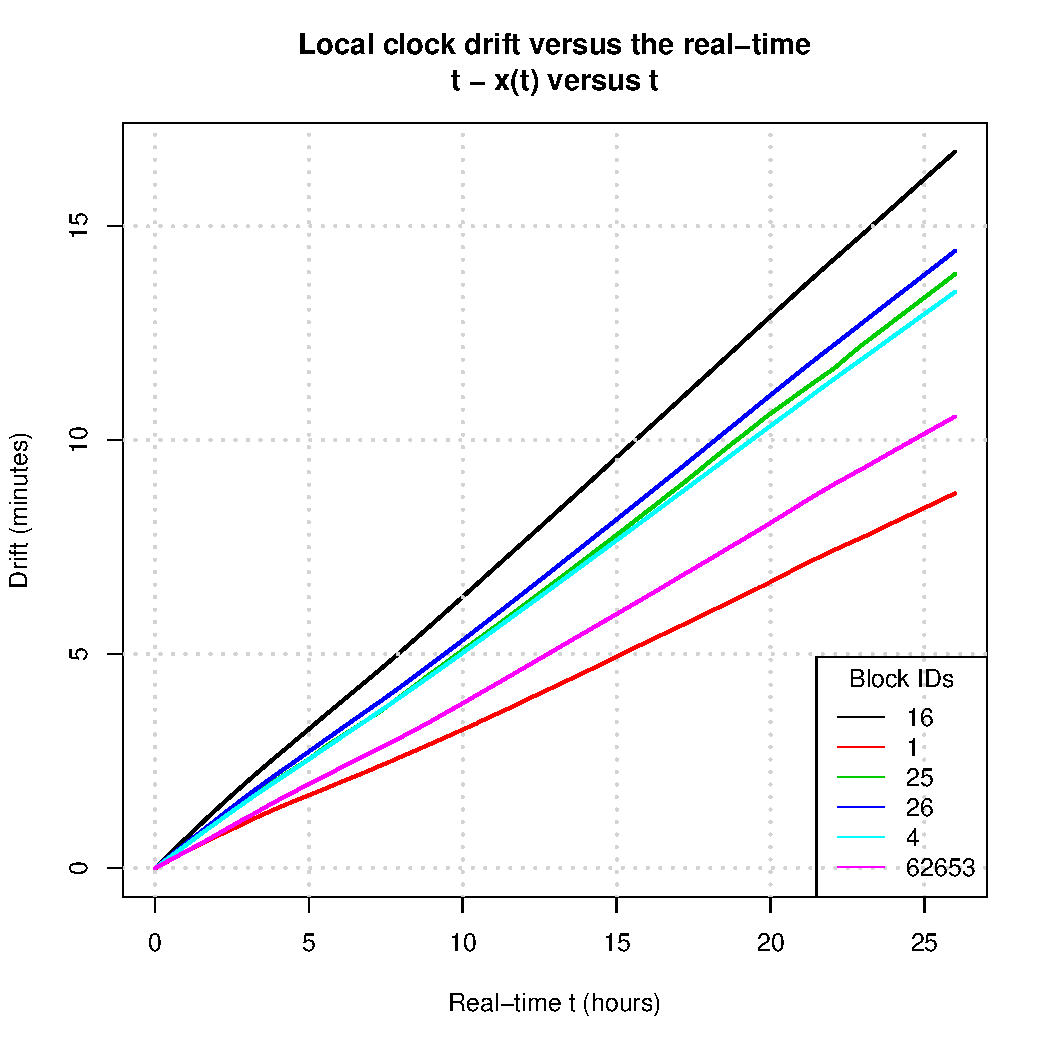
\includegraphics[width=0.45\textwidth]{pictures/drift.pdf}
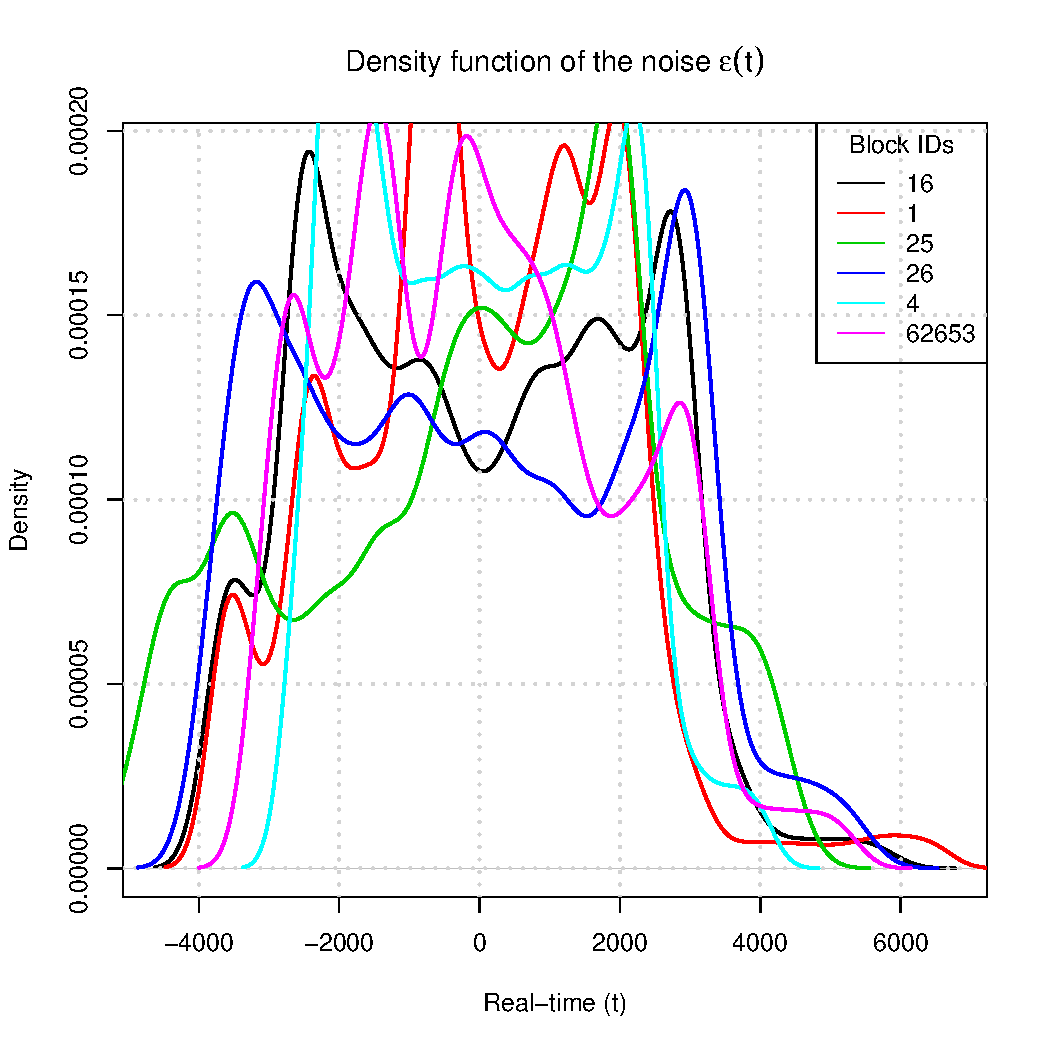
\includegraphics[width=0.45\textwidth]{pictures/noise.pdf}
\caption{Local clock drift (t - x(t)) and noise ($\epsilon(t)$) distribution.}
\label{fig:drift-noise}
\end{figure}

\begin{figure}[h!]
\footnotesize
\begin{center}
\begin{tabular}{|c|c|c|c|c|} 
\hline
Parameter & Min & Mean & Max & Standard-deviation \\
\hline
$D$ & 1.613992e-11 & -1.179717e-11 & -7.991859e-12 & 3.060884e-12 \\
\hline
$y_0$ & 0.9896537 & 0.9922277 & 0.9949096 & 0.001851285\\
\hline
$x_0$ & -5984.141 & -3532.051 & -785.9812 & 1921.629\\
\hline
Residual standard error & 1688.103 &  2080.197  & 2423.646 & 294.832\\
\hline
\end{tabular}
\end{center}
\caption{Parameters}
\end{figure}

\begin{figure}[h!]
\centering
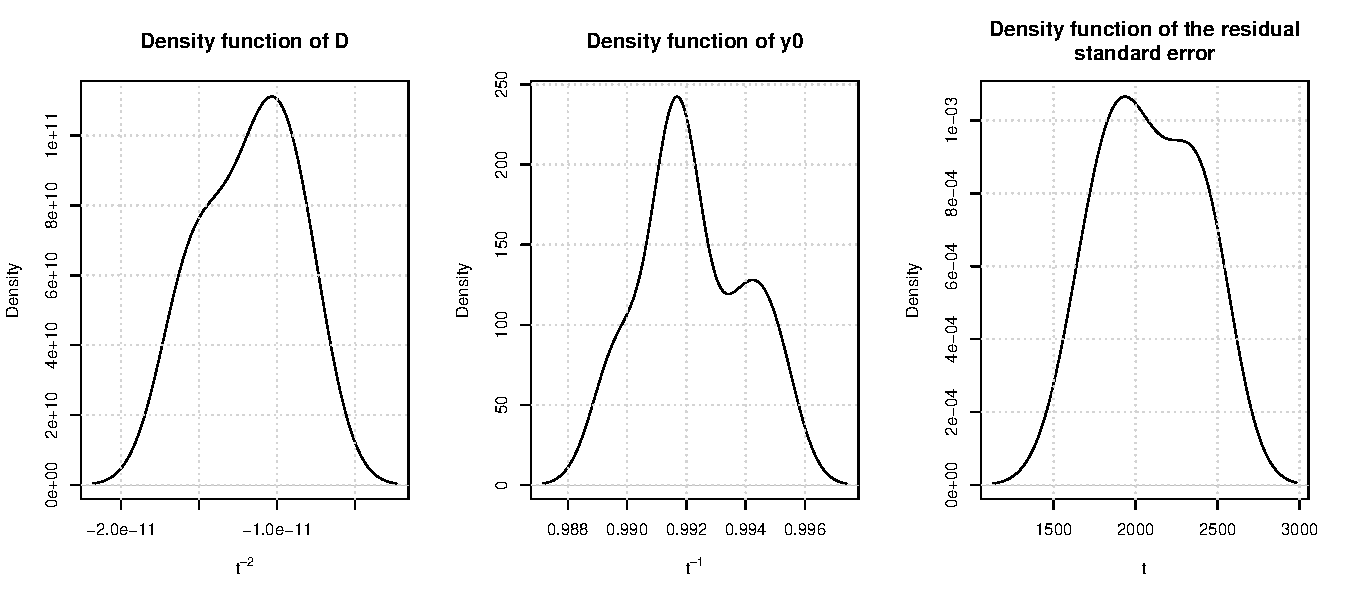
\includegraphics[width=0.70\textwidth]{pictures/parameters.pdf}
\caption{Parameter distributions.}
\label{fig:drift-noise}
\end{figure}

The parameters $D$, $y_0$ and the residual standard error seems normally distributed. As a consequence, we randomly generate clock parameters according to normal laws with the correspong mean and standard deviation.

\subsection{Clock simulation in DES}

\cite{ring2010clock} explains how to enhance DES with efficient local clock simulation.

\newpage

\bibliographystyle{plain}
\bibliography{manual}

\end{document}
